\documentclass[../notes.tex]{subfiles}
\graphicspath{{\subfix{../img/}}}
\begin{document}

\part{ECE360: Electronics}

\marginnote{Taught by Prof. Khoman Phang}

\section{Admin and Preliminary}

\subsection{Lecture 1}



\subsubsection{Mark Breakdown}

\begin{table}[H]
	\centering
	\caption{Mark Breakdown}
	\begin{tabular}{|c|c|}
		\hline
		Test 1 & 15 \\
		Test 2 & 20 \\
		Homework & 10 \\
		Labs & 12 \\
		Final & 43 \\
		\hline
	\end{tabular}
\end{table}

\subsubsection{Diodes}

Diodes are an electronic valve which causes current to only flow in one direction.
An ideal diode is an open circuit in the closed direction and a closed circuit in the other, so the current is always in the direction of the arrow (+'ve @ arrow base, -'ve at arrow point)\sn{recall: passive sign convention}.


\begin{figure}[H]
	\centering
	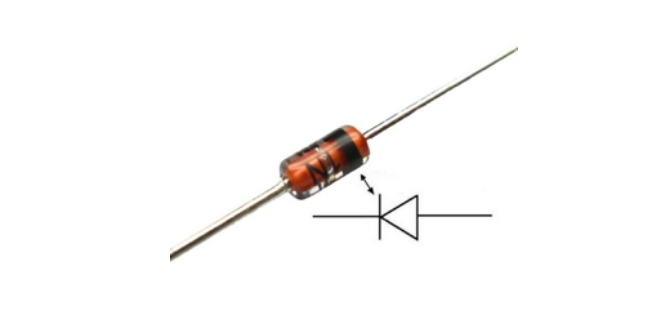
\includegraphics[width=0.8\linewidth]{img/360_diode.png}
	\caption{A diode and its symbol}
	\label{fig:360:diode}
\end{figure}


An example of a diode circuit is the half-wave rectifier which turns an AC signal to a DC signal \marginnote{Can take oscilloscope over resistor to see that a pure DC signal has been generated}

\begin{figure}[H]
	\centering
	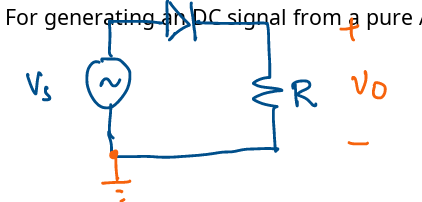
\includegraphics[width=0.8\linewidth]{img/image_2022-09-09-12-51-30.png}
\end{figure}

\begin{figure}[H]
	\centering
	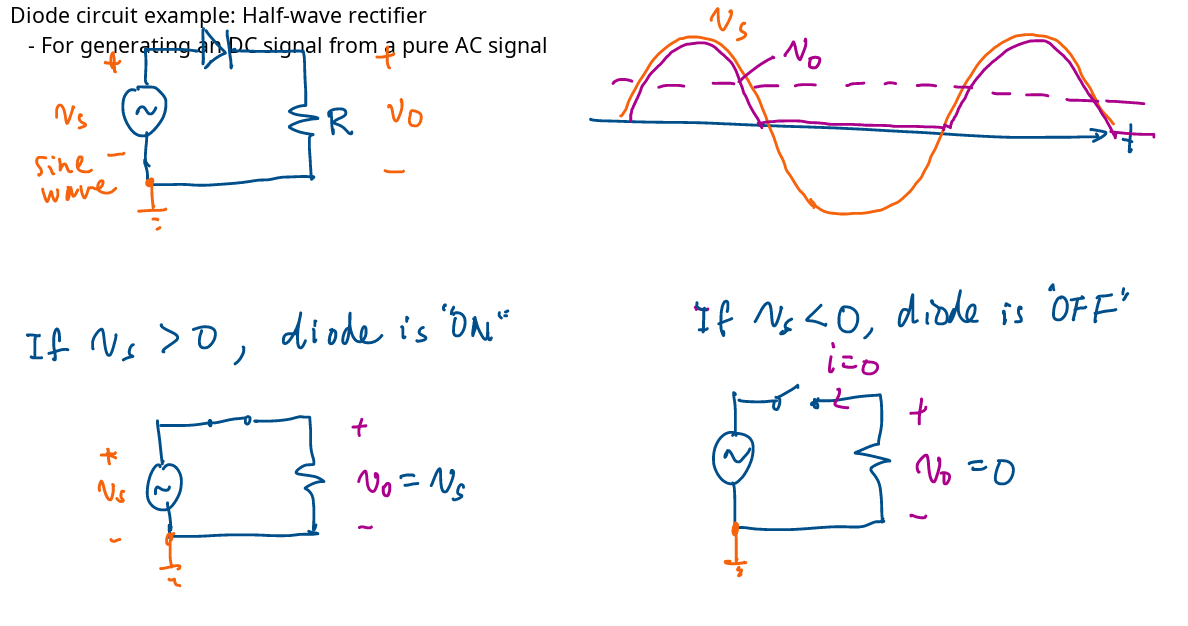
\includegraphics[width=0.8\linewidth]{img/image_2022-09-09-13-01-02.png}
\end{figure}

\section{Diodes}

\subsection{Lecture 2}

More formally, off/on for diodes should be referred to as:
\begin{itemize}
	\item Off $ \leftrightarrow $ reverse bias
	\item On $ \leftrightarrow $ forwards bias
\end{itemize}

\begin{figure}[H]
	\centering
	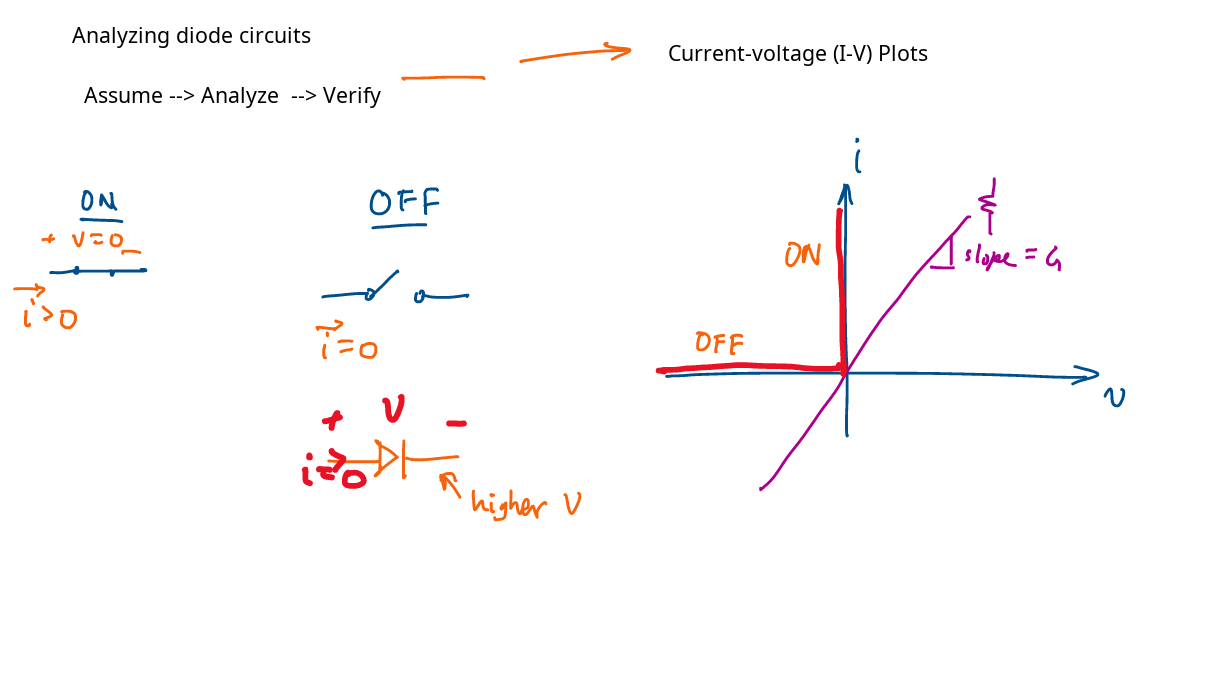
\includegraphics[width=0.8\linewidth]{img/image_2022-09-12-09-41-11.png}
	\caption{General steps for analyzing non-linear circuits. Note plotting out expected response}
\end{figure}





\marginnote{An example of how this is used in circuit design is to manage two power sources. Consider an Arduino that could be powered by an AC adapter or by a computer's USB port. This circuit would choose the higher voltage source and prevent backflow into the other power source due to any potential power differentials. It is also effectively an OR gate}
\begin{figure}[H]
	\centering
	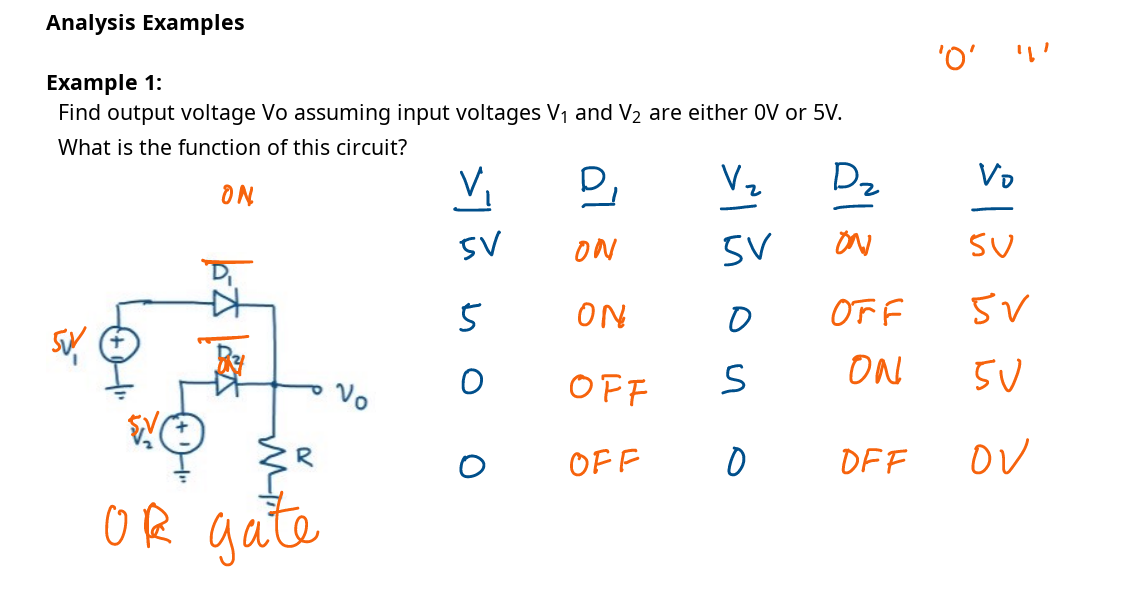
\includegraphics[width=0.8\linewidth]{img/image_2022-09-12-09-54-03.png}
\end{figure}




\begin{figure}[H]
	\centering
	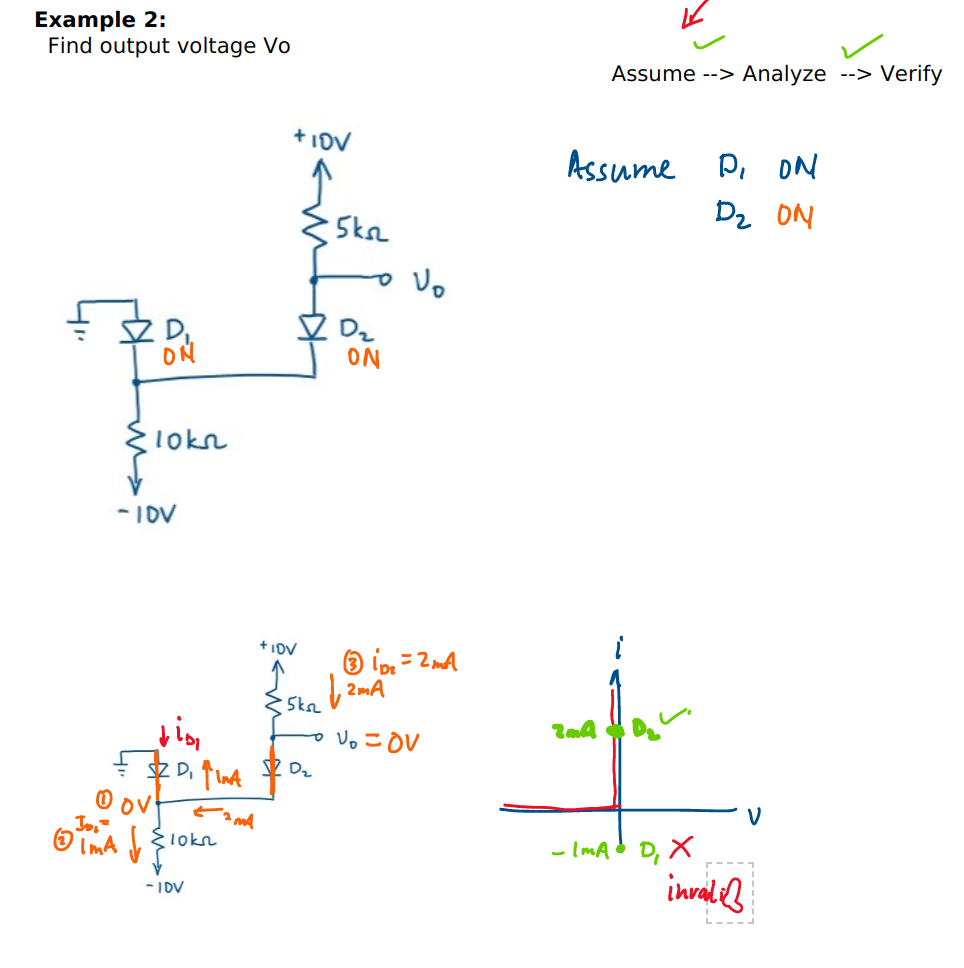
\includegraphics[width=0.8\linewidth]{img/image_2022-09-12-10-02-42.png}
\end{figure}

In this example the initial assumption was incorrect. 

Let's try another analysis with $ D_1  $ off and $ D_2 $ on:

\begin{figure}[H]
	\centering
	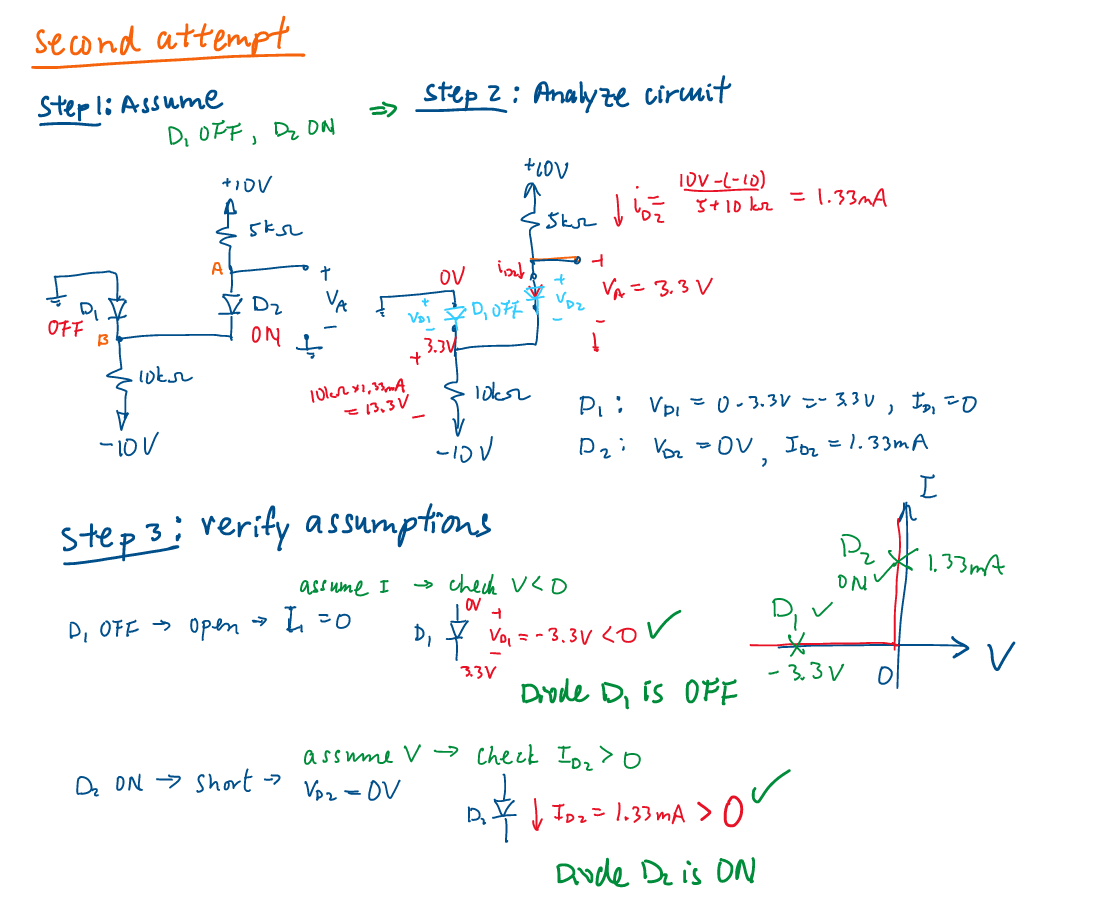
\includegraphics[width=0.8\linewidth]{img/image_2022-09-13-13-20-51.png}
\end{figure}

If we were to do this brute force we'd have to consider 4 cases, so it's important to build up some sort of intuition for the circuit.


\subsection{Lecture 3}


Today we're going to look at the characteristics of real diodes.



\begin{figure}[H]
	\centering
	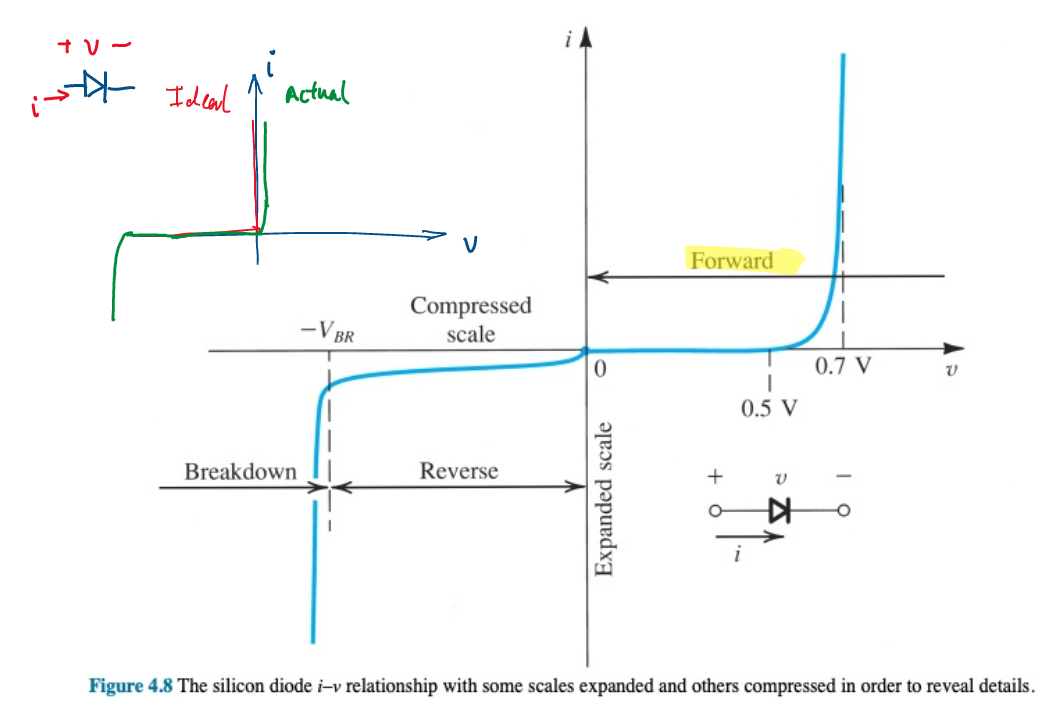
\includegraphics[width=0.8\linewidth]{img/image_2022-09-13-13-26-58.png}
\end{figure}

Real diodes have a little bit of leakage current and also encounter a breakdown point where they're no longer able to block the current.

\begin{theorem}
	\textbf{Forward Bias} 

	\begin{equation}
		i = I_s(e^{\frac{V}{V_T} - 1})
		\label{eq:360:forward_bias}
	\end{equation}

	Where:
	\begin{equation}
		V_T = \frac{kT}{q} \quad [V]
	\end{equation}
	\marginnote{$ k $ is Boltzmann's constant, $ T $ is temperature in Kelvins, $ q $ is the charge of an electron.}

	Most of the time we can assume that the circuit is at room temperature and that $ v_T = 25mV $.
	Note that this value explodes when $ V > V_T  $ which is the breakdown point.
	When encountering a reverse bias $ V_s < 0 $, the $ -1 $ term comes in and causes $ i \approx I_s  $  \marginnote{$ I_s $ is the scale current which is usually $ \approx 1pA $, which doesn't change much until the breakdown point.}

	The scale current is just a general constant which varies in range from $ 10^{-9} to 10^{-15} A $ and scales with temperature, doubling with every approximately $ 5^o C $ increase in temperature.





	Note: the ideal diode equation can be rearranged to find an expression for voltages

	\begin{equation}
		V = V_T \ln{(\frac{i}{I_s}) = \ln{(10)} V_T \log_{10}{(\frac{i}{I_s})}}
		\label{eq:360:forward_bias_v}
	\end{equation}

	These expressions turns out to be quite reliable for reasonable diodes to reasonable voltages.

\end{theorem}

Using the ideal diode equation we can find the relationship between voltages and currents as they pass through the diode.


\begin{equation}
	\frac{i_2}{i_1} = \frac{I_s e^{\frac{V_2}{V_T}}}{I_s e^{\frac{V_1}{V_T}}} = e^{\frac{V_2 - V_1}{V_T}}
\end{equation}


\begin{equation}
	V_2 - V_1 = V_T \ln{(\frac{i_2}{i_1})} \xrightarrow{\text{room temperature}} 60mV \log_{10} \frac{i_2}{i_1}
\end{equation}





\begin{example}
	\begin{figure}[H]
		\centering
		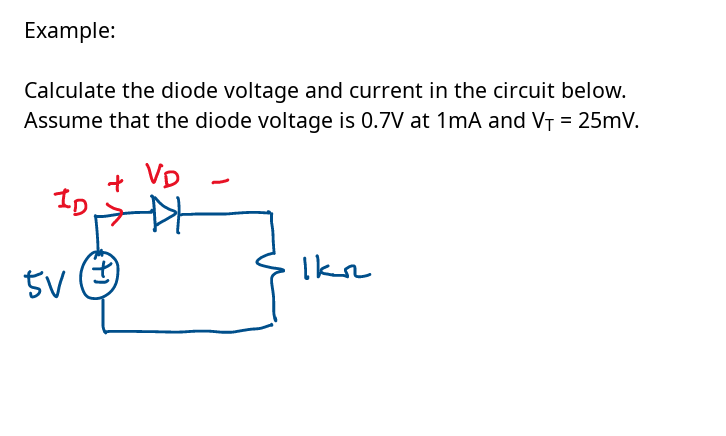
\includegraphics[width=0.8\linewidth]{img/image_2022-09-13-13-55-18.png}
	\end{figure}

	Recall \eqref{eq:360:forward_bias}. Plugging in the given values gives us the scale current.

	\begin{equation}
		1mA = I_s e^{\frac{0.7V}{25mV}}, I_s = 6.9 \cdot 10^{-16} A \Rightarrow I_o = I_s e^{v_o/v_T}
	\end{equation}

	Ohm's law can then be applied at the resistor

	\marginnote{$ V_D $ is the voltage across the diode }

	\begin{equation}
		V_r = IR = I_oR  = 5V - V_D \Rightarrow 5 - V_D = I_o R
	\end{equation}

	So we have two equations and two unknowns (since we know $ v_T = 25mV $ but $ v_o $ was used at first just to find $ I_s $ ) Solving for the unknowns gives us:

	\begin{itemize}
		\item $ V_o  = 0.736 V $
		\item $ I_D = 4.264 mA $ 
	\end{itemize}
\end{example}


\section{Lecture 4 \& 5: Forward conducting diodes}
	\marginnote{$ V_{DD} $ is DC voltage, $ v_D $ is small signal voltage, $ V_D $ is the diode voltage}


The exponential model accurately describes the diode outside of the breakdown region, though it's nonlinear behaviour makes it difficult to use.

For $ V_{DD} > 0.5V $

\begin{equation}
	I_D = I_S e^{V_D/V_T}
	\label{eq:360:forward_conducting_diode}
\end{equation}

Where 
\begin{itemize}
	\item $ I_S $ is the diode parameter
	\item $ V_T $ is the thermal voltage
\end{itemize}

Another equation may be produced via Kirchhoff's law

\begin{equation}
I_D = \frac{V_{DD} - v_d}{R}
 \label{eq:360:forward_conducting_diode_kirchhoff}
\end{equation}



The unknown quantities $ I_D $ and $ v_d $ may be solved for via graphical analysis or iteration.

\begin{example}

	This simple circuit is used to demonstrate the exponential model of the diode.
	\begin{figure}[H]
		\centering
		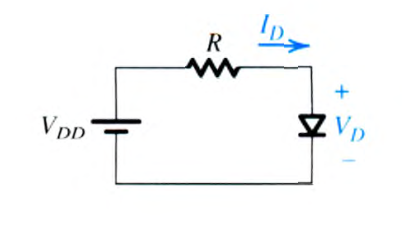
\includegraphics[width=0.8\linewidth]{img/image_2022-09-16-22-33-11.png}
		\caption{Simple example circuit with diode}
		\label{fig:360:forward_conducting_diode_example}
	\end{figure}
	
	Plots of the diode characteristics and Kirchhoff's relation are plotted, the intersection of which gives the solution.

	\begin{figure}[H]
		\centering
		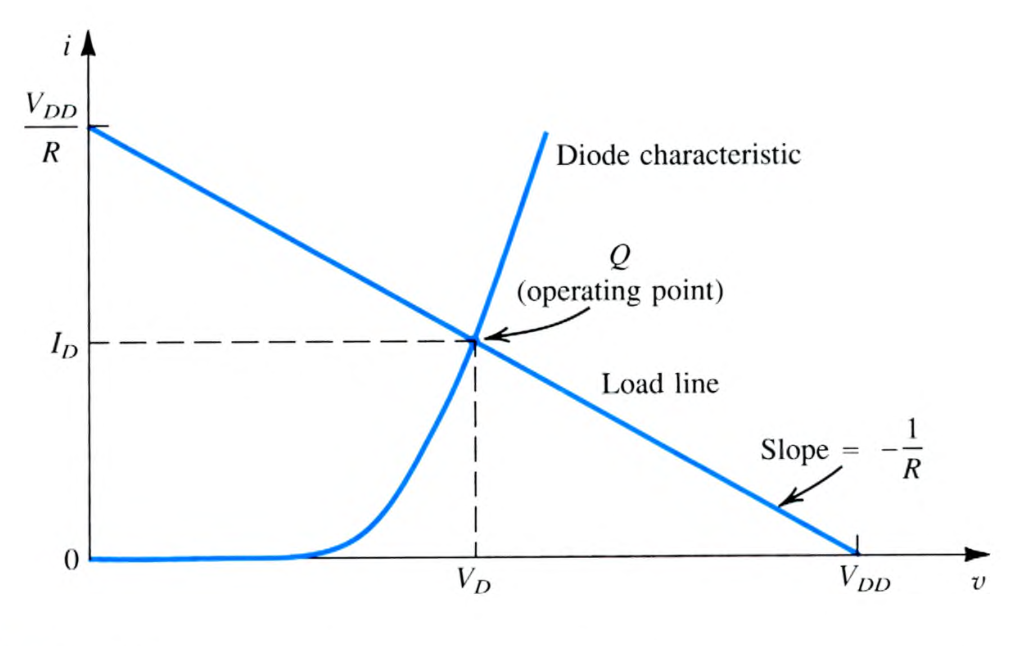
\includegraphics[width=0.8\linewidth]{img/image_2022-09-16-22-32-51.png}
	\end{figure}
\end{example}

An iterative procedure may also be applied to solve for the unknowns, the procedure for which will be illustrated through an example


\begin{example}

	Find $ I_D, V_D $ for the circuit in the previous example (Fig.~\ref{fig:360:forward_conducting_diode_example}). $ V_{DD} = 5V, R = 1k\Omega $, and at $ V_{D} 0.7V$,  $I_D = 1mA $ 


\begin{enumerate}
	\item Assume $ V_D = 0.7V$, then use \eqref{eq:360:forward_conducting_diode_kirchhoff} to find $ I_D $.
		\begin{equation}
			I_D = \frac{5V - 0.7V}{1k\Omega} = 4.3mA
		\end{equation}
		
	\item Use the diode equation \eqref{eq:360:forward_conducting_diode} to get a better estimate for $ V_D $.

		\begin{equation}
			V_2 - V_1 = 2.3 V_T \log \frac{I_2}{I_1} \Rightarrow V_2 = V_1 + 0.06 \log \frac{I_2}{I_1}
		\end{equation}
	substituting $ V_1 = 0.7V, I_1 = 1mA, I_2 = 4.3mA $,
	\begin{equation}
		V_2 = 0.738V \Rightarrow I_D = 4.3mA, V_D = 0.738V
	\end{equation}
	\begin{itemize}
		\item This states that for a decade\mn{Factor of 10} change in current the diode voltage drop changes by $ 2.3(V_T \approx 60mV) $ which is negligibly small for $ v < 0.5V $. 
		The voltage at which the this behaviour becomes significant is called the \textbf{cut-in voltage} 
	\end{itemize}

\item Repeat steps 1 and 2 with the new values until the values more or less become stable
\end{enumerate}
\end{example}

This iterative model is powerful and yields accurate results, but can be computationally expensive especially when calculating by hand.
To address this we employ other models such as the \textit{constant-voltage-drop} model which approximates the exponential characteristics via a piecewise linear model.
The reason why this is possible is because forward conducting diodes exhibit a voltage drop that varies in a relatively narrow range.

\begin{figure}[H]
	\centering
	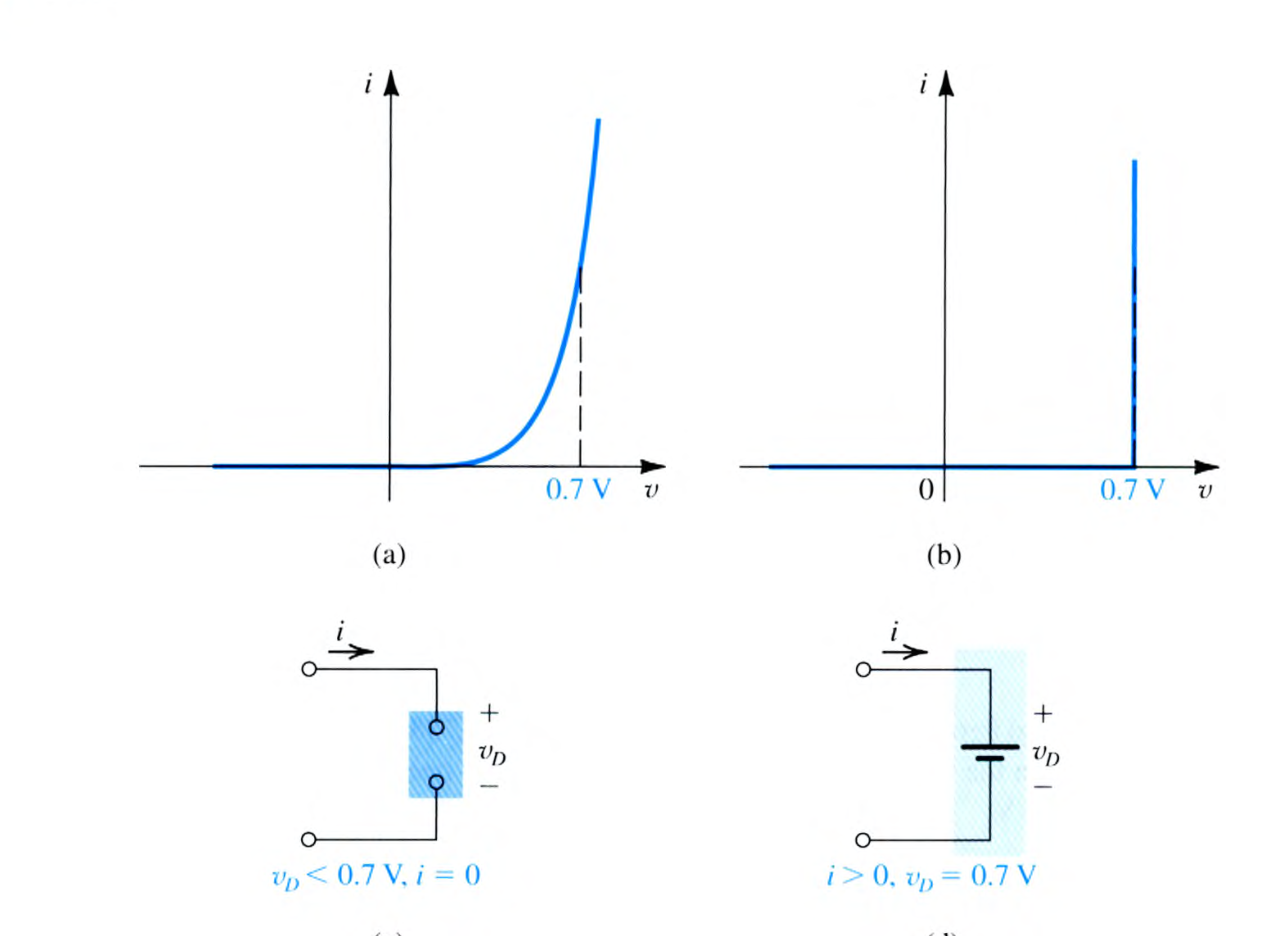
\includegraphics[width=0.8\linewidth]{img/image_2022-09-16-22-49-19.png}
\end{figure}


Using the constant voltage drop model in our analysis looks the same as before, but with $ V_D $ directly taking on the value of $ 0.7V $ (as per the prior example) instead of being solved for with the diode equation.



In applications that involve voltages greater than the voltage drop (i.e. usually $ \approx 0.6-0.8V $  ) we can neglect the diode voltage drop altogether while calculating the diode current.

\begin{equation}
	\begin{split}
		V_D &= 0V \\
		 I_D &= \frac{5-0}{1} = 5mA  \\
	\end{split}
\end{equation}



This is generally good enough for a first estimate, though the previous model isn't that much more work and gives more accurate results.
The primary use of this model is to determine which diodes are on or off in a multi-diode circuit


\section{Small-Signal Model}


The small signal method is an alternative model used to describe the nonlinear diode's characteristics with greater accuracy than piecewise linear models\marginnote{Similar methods will be applied to transistors in later chapters}.


Consider a small $ \Delta V_{DD} $ applied to the diode, which would cause a small $ \Delta I_D, \Delta V_D $.
We want to find a quick way of determining the values of these incremental changes.

\begin{figure}[H]
	\centering
	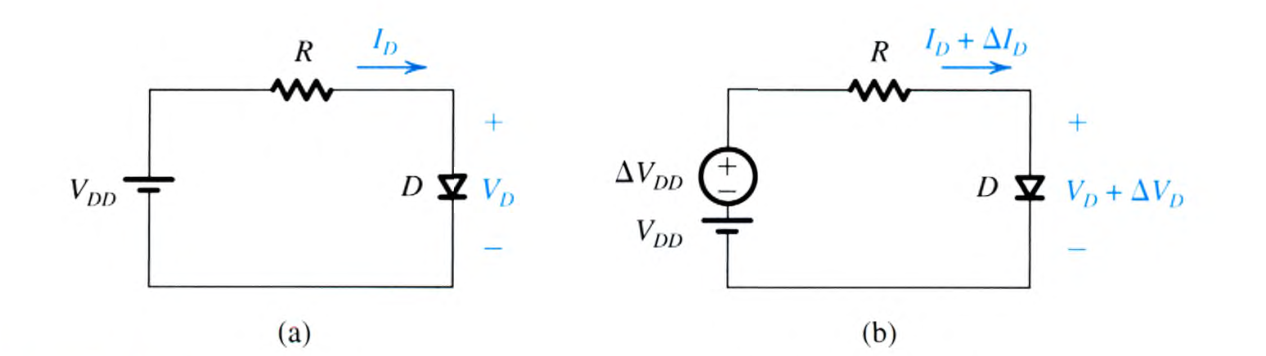
\includegraphics[width=0.8\linewidth]{img/image_2022-09-16-23-15-07.png}
\end{figure}

Skipping a bunch of math\sidenote{It is 11:17pm and I have two more lectures to catch up to today} the results are as follows:
\sidenote{Small signal analysis can be performed separately from the dc bias analysis because of the linearization of diode characteristics in the small-signal approximation}

\begin{definition}
	\textbf{Small signal approximation}
	\begin{equation}
		i_D(t) \approx I_D (1+ \frac{v_d}{V_T} )
	\end{equation}
	This is valid for when variations in diode voltage $ |v_d| \lessapprox 5mV$.


	\begin{equation}
	 r_d = \frac{V_T}{I_D} 
	 \label{eq:360:small_signal_diode_resistance}
	\end{equation}
	From this we can define the small signal resistance as the resistance relating $ i_d $ to $ v_d $
	
\end{definition}



The steps for calculating the small signal model are as follows:

\begin{enumerate}
	\item Perform a dc analysis using the exponential, constant-voltage-drop, or piecewise-linear model.
	\item Linearise the circuit. For a forward-based diode, find $ r_d $ by substitution $ I_D $   into \eqref{eq:360:small_signal_diode_resistance}. The small-signal equivalent circuit is found by eliminated all independent dc sources\sidenote{since we already accounted for them in step 1} and replacing the diode with its small-signal resistance $ r_d $ 
	\item Solve the linearised circuit. In particular we would want to find $ \Delta I_D, \Delta V_D $ and check to see if it is consistent with our approximation, i.e. that $ \Delta V_D \lessapprox 5mV $ 
\end{enumerate}

The reason why we linearise these non-linear systems, we, as engineers, try to linearise them because it is convenient to be able to use superposition, phasors, Fourier series, Laplace transforms, and so forth.


\section{Lecture 6: Small signal model, cont'd}


$ V_D $ can be thought of an input to a transfer function that is the diode, with $ I_D $ being the output. 
If the input signal is more or less a triangular wave the output will be as well.

\begin{figure}[H]
	\centering
	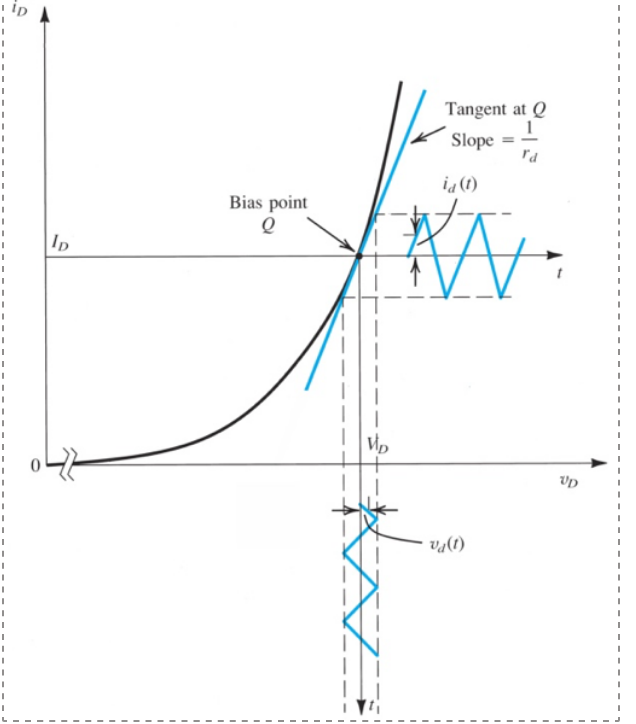
\includegraphics[width=0.5\linewidth]{img/image_2022-09-20-13-17-59.png}
\end{figure}

Since we are applying a linear approximation, superposition may apply;

\begin{equation}
	f(a+b+c\ldots) = f(a) + f(b) + f(c) + \ldots
\end{equation}


Here we can think of the function as

\begin{equation}
	f(V_o  + v_d) = f(V_o) + f(v_d)
\end{equation}

Small signal analysis works because, by superposition, we can zero out the other sources ($ V_o $, etc ) and inspect only the effect of the small signal voltage on the system.



\subsubsection{Deriving small-signal resistance}

\begin{figure}[H]
	\centering
	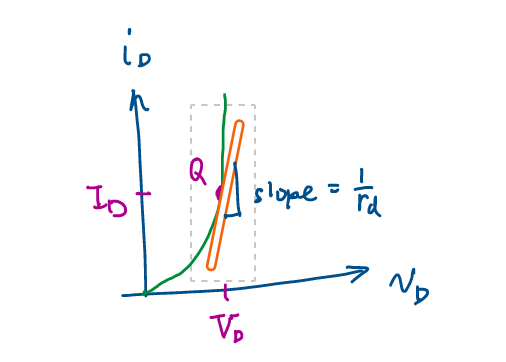
\includegraphics[width=0.8\linewidth]{img/image_2022-09-20-13-28-41.png}
\end{figure}

Resistance can be found as the slope of the $ I-V $ relationship. 
The following is a proof of~\eqref{eq:360:small_signal_diode_resistance}.

\begin{proof}
\begin{equation}
	i_D = I_s e^{ \frac{V_D}{V_T} }
\end{equation}

\begin{equation}
	\text{slope} = \frac{di_D}{dv_o}  = I_S (\frac{1}{v_T}) e^{\frac{V_D}{V_T} }
\end{equation}

Then, substitute values at the operational point $ Q $ , i.e. $ I_D, V_{DD} $ 

\begin{equation}
	\text{slope} = I_S e^{V_D / V_T} (\frac{1}{V_T}) \implies \frac{I_D}{V_T} = \frac{1}{r_d}
\end{equation}

And therefore
\begin{equation}
	r_d = \frac{V_T}{I_D}
\end{equation}

\end{proof}


\begin{enumerate}
	\item Calculate DC bias point $ Q $ 
	\item Derive small-signal circuit
	\item Analyze small-signal circuit
	\item If required, recombine to arrive at final result
\end{enumerate}

\begin{figure}[H]
	\centering
	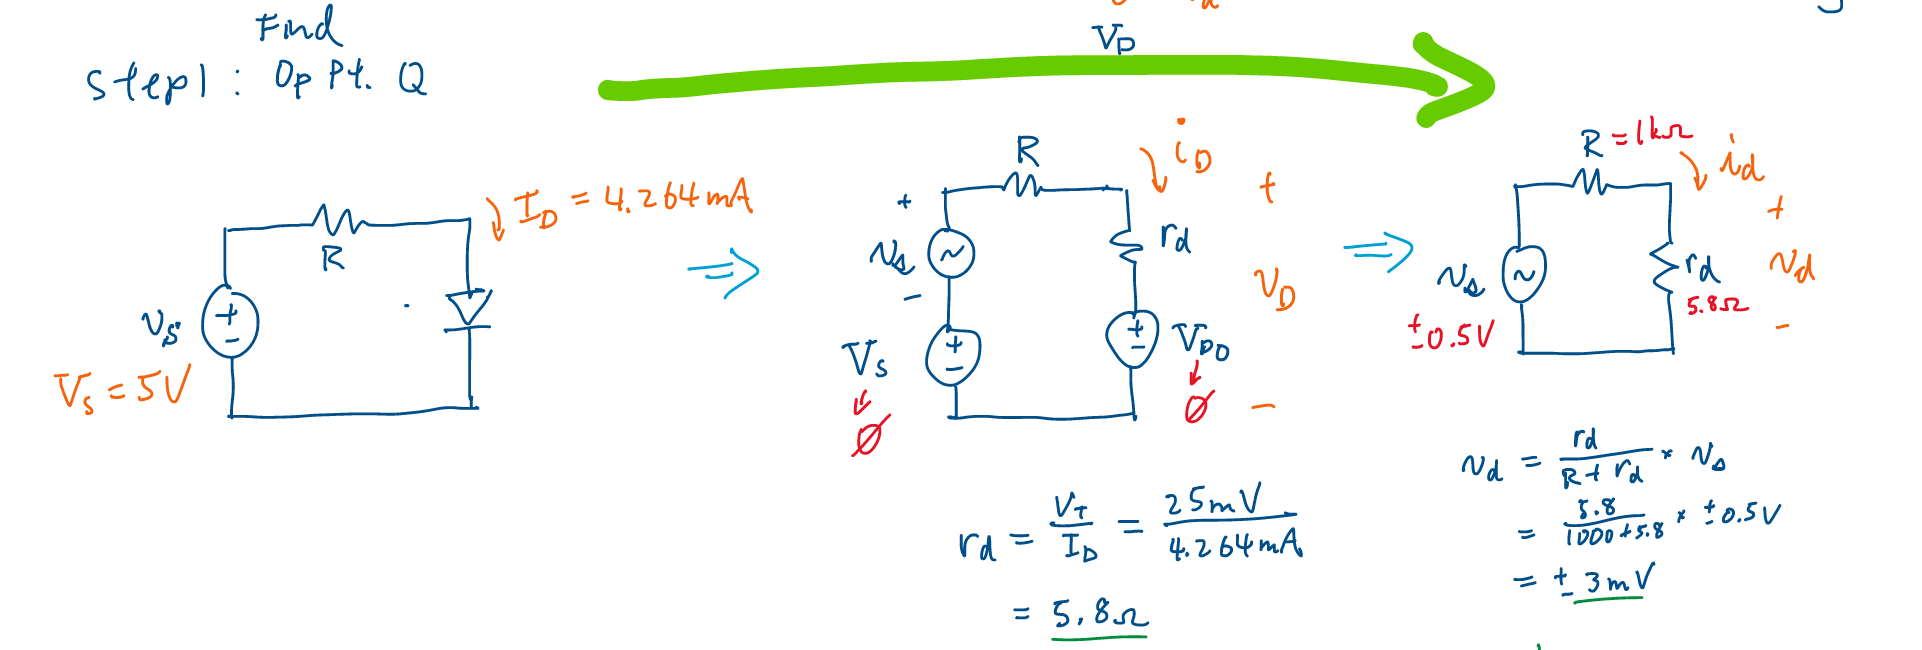
\includegraphics[width=0.8\linewidth]{img/image_2022-09-20-13-41-57.png}
\end{figure}


The textbook skips the middle step where we actually apply the small signal approximation and all the values have not been offset by the bias point yet.
Note that voltages/values in the 3rd step (small signal approx) are all relative to the bias point $ Q $ .





Applying this to our circuit we find

\begin{equation}
	r_d = \frac{V_T}{I_D} = \frac{25mV}{4.264mA} = 5.8 \Omega
\end{equation}

This was not as accurate as the exponential model but it is more than close enough 99\% of the time.
But also the $ 0.7V $ constant voltage drop model is usually sufficient as well.


\begin{proof}

	The small-signal approximation is valid for voltage variations up to $ \pm 5mV $ 
	\begin{equation}
		\begin{split}
			i_D &= I_S \exp (V_D / V_T)  \\
			&= I_S \exp \frac{V_DD + v_d}{V_T}  \\
			&= I_D \times e^{v_d/v_T} \\
		\end{split}
	\end{equation}

	$ e^x  $  can be expanded to a power series

	\begin{equation}
		\begin{split}
			e^x &= 1 + x + \frac{x^2}{2!} + \frac{x^3}{3!} + \ldots \\
			 &\approx 1+x \qquad \text{if } \frac{x^2}{3!} \ll x \rightarrow x \ll 2 \\
		\end{split}
	\end{equation}

	Therefore $ \frac{v_d}{V_T} \ll 2 $, so $ v_d \ll 2V_T = 50mV $ 

	So make 

	\begin{equation}
		|v_d| < 5mV
	\end{equation}
	
	
\end{proof}

In the lab we'll be using a variable attenuator circuit, which involves a voltage source
Can make a current source with a voltage source and a large resistor.

\begin{figure}[H]
	\centering
	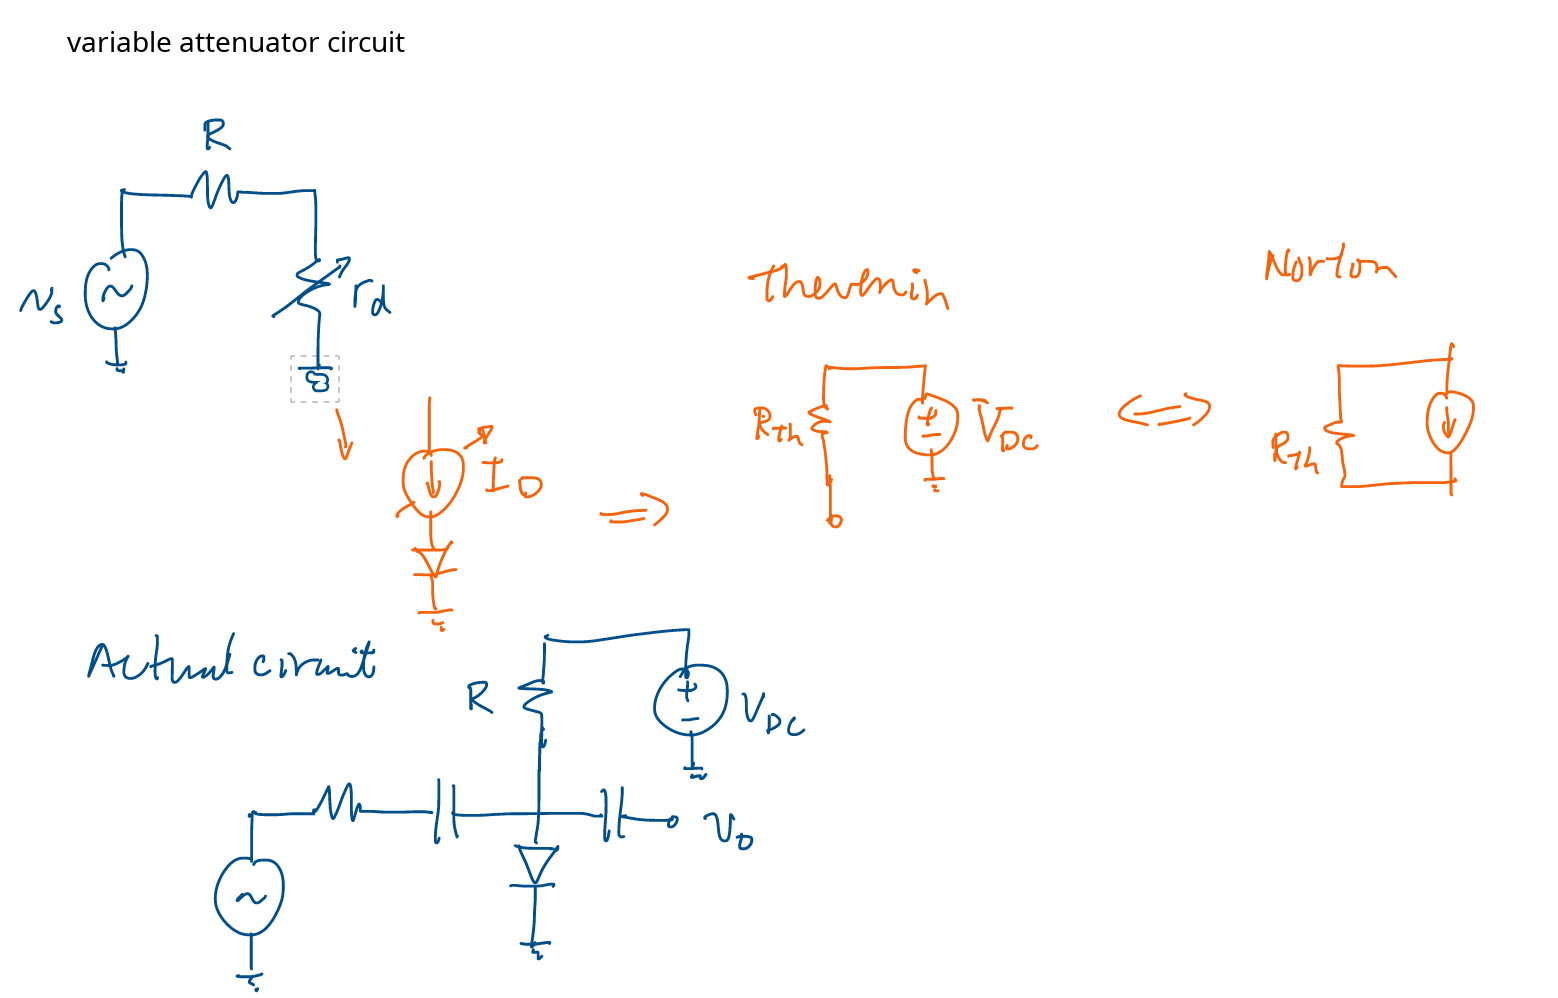
\includegraphics[width=0.8\linewidth]{img/image_2022-09-20-14-02-07.png}
\end{figure}

This will be covered more next lecture. TLDR: can use small signals and then build up a circuit to get the intended $ Q $ using biases.



% TODO(ihasdapie): Double check $ V_DD, v_d, V_D $ usage across these notes.







\section{Lecture 7}

Let's take a deeper look into the variable attenuator circuit discussed last class.


\begin{figure}[H]
	\centering
	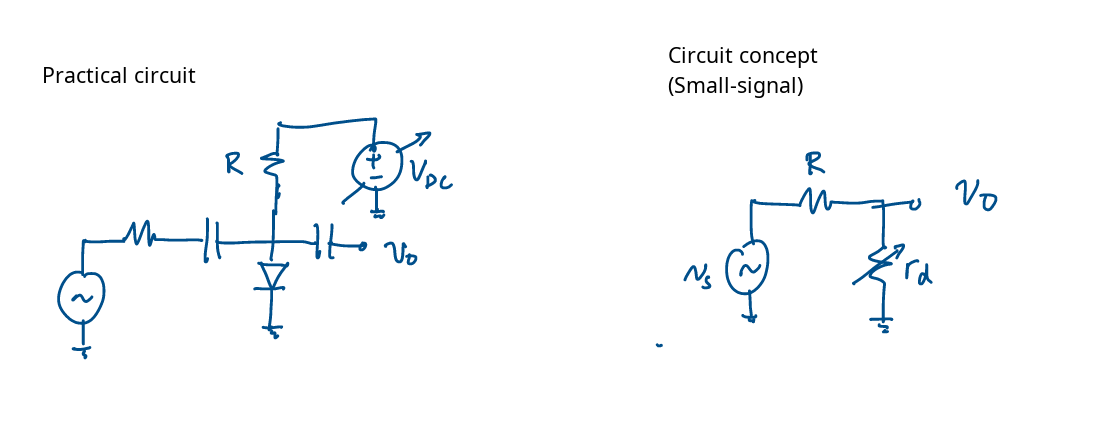
\includegraphics[width=0.8\linewidth]{img/image_2022-09-23-12-20-50.png}
\end{figure}

\begin{itemize}
	\item The capacitors in this circuit can be treated like short circuits because they are large (which is why we don't see them in the small-signal circuit).
	\item The constant voltage offset source gets zeroed out in the small-signal circuit because it is a constant, thereby becoming a ground.
	\item Current sources become open circuits
	\item Negative currents 
\begin{figure}[H]
	\centering
	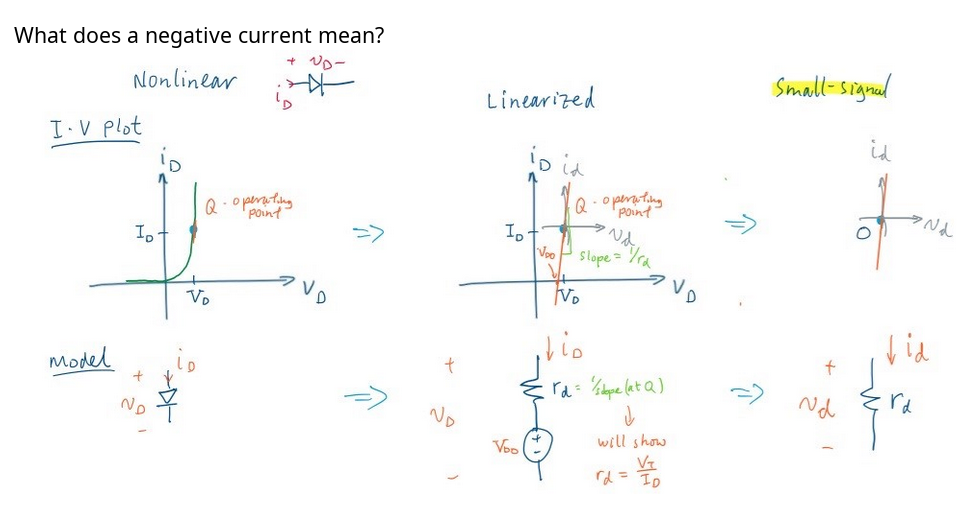
\includegraphics[width=0.8\linewidth]{img/image_2022-09-23-12-33-13.png}
\end{figure}

\end{itemize}



\marginnote{Most of the homework, etc we will be practicing working from the practical circuit to the small-signal design, whereas as a designed we will usually be going the other way around.}

\section{Rectifiers}

We have previously talked about the half-wave rectifier circuit, which used a single diode to rectify a waveform to only the positive values

\begin{figure}[H]
	\centering
	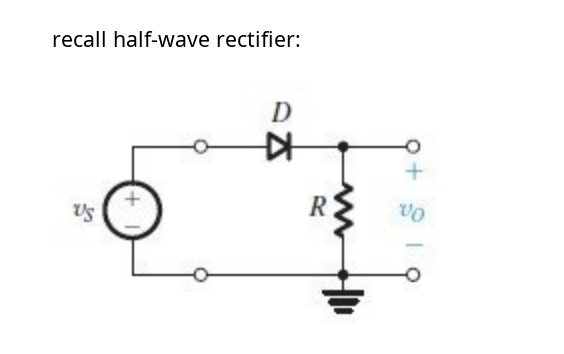
\includegraphics[width=0.8\linewidth]{img/image_2022-09-23-12-41-12.png}
\end{figure}

This isn't very efficient because it only uses half of the waveform, so it is desirable to build a \textit{full wave} rectifier

\begin{figure}[H]
	\centering
	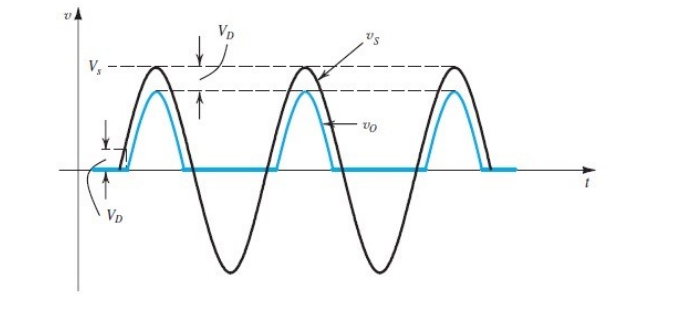
\includegraphics[width=0.8\linewidth]{img/image_2022-09-23-12-41-30.png}
\end{figure}


What we want with a full-wave rectifier is to automatically interchange the wires whenever the input signal goes from negative to positive and vice-versa as to provide the load a wholly positive signal.



A full wave rectifier can be built as follows

\begin{figure}[H]
	\centering
	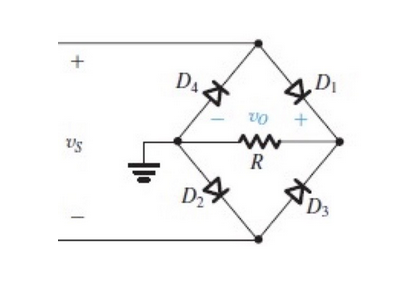
\includegraphics[width=0.8\linewidth]{img/image_2022-09-23-12-48-48.png}
	\caption{When the signal is positive it will flow from diode 1 to the load and then to diode 2. When it is the negative polarity it will go through diode 3 to the load and then return through diode 4. Note how the direction remains the same, and how we selectively connect the ground to the top or bottom terminal depending on the input polarity.}
\end{figure}


\begin{figure}[H]
	\centering
	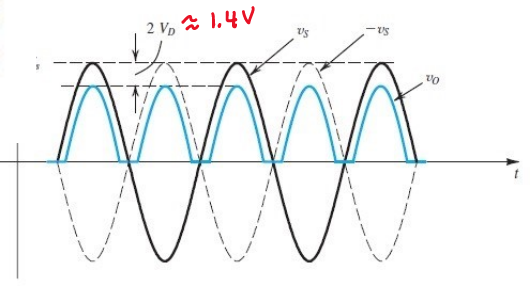
\includegraphics[width=0.8\linewidth]{img/image_2022-09-23-12-52-41.png}
	\caption{Comparing the two there is a little more loss but at least we get the full wave now}
\end{figure}


A \textbf{peak rectifier} uses a capacitor as an energy storage device to hold the voltage at the peak value.

\begin{figure}[H]
	\centering
	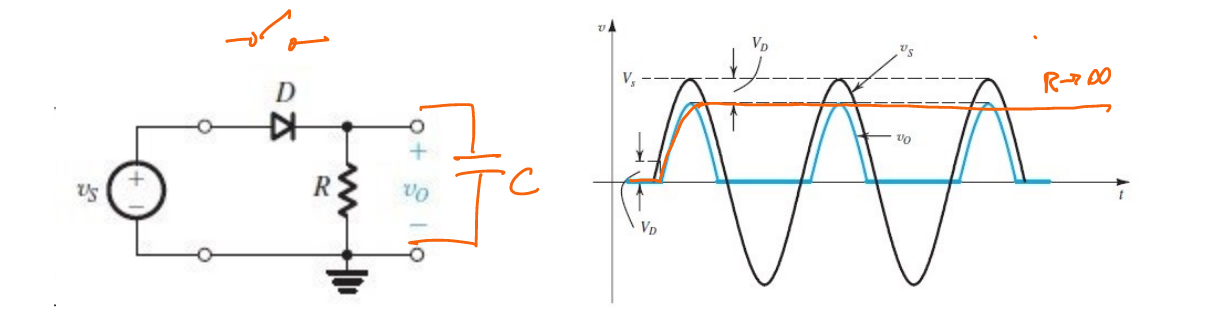
\includegraphics[width=0.8\linewidth]{img/image_2022-09-23-12-58-46.png}
	\caption{Capacitor size and frequency must be tuned as to avoid voltage drop (recall RC circuits. Note that the time constant $ \propto RC $, so a bigger resistor (slower rate of discharge) or bigger capacitor (bigger energy storage) can reduce voltage drop)}
\end{figure}


\subsection{Lecture 8}
Hard limiting circuits include a pair of diodes which cause only a maximum of $ 0.7V $ signal to pass through.

\begin{figure}[H]
	\centering
	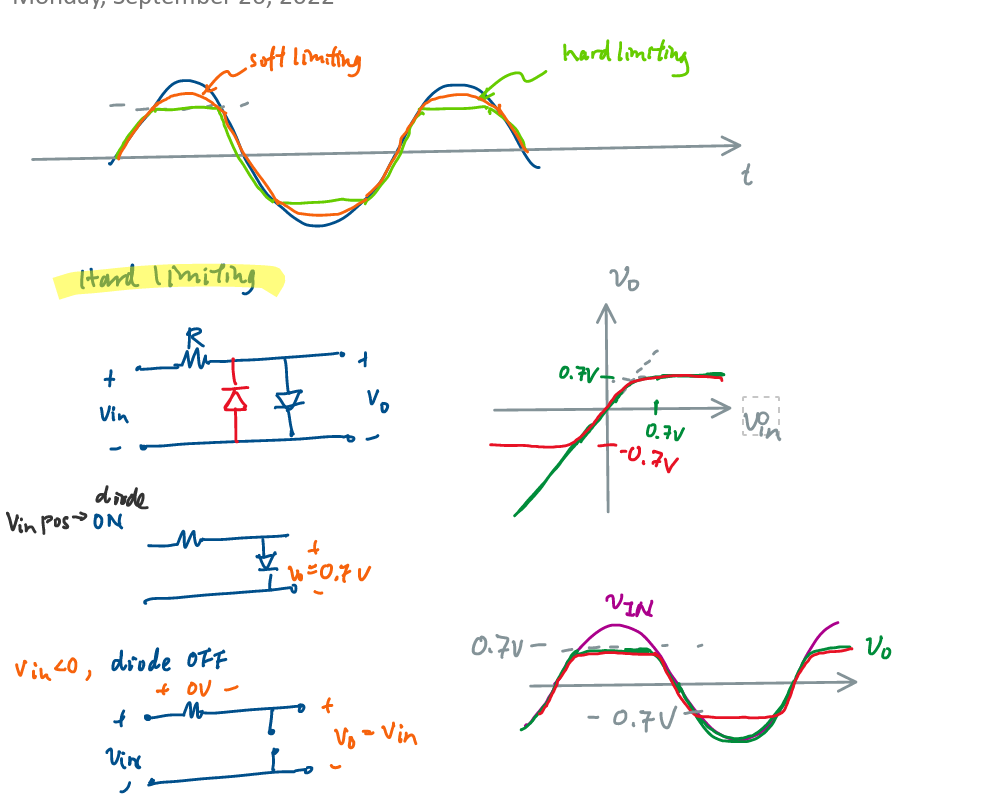
\includegraphics[width=0.8\linewidth]{img/image_2022-09-26-12-35-18.png}
\end{figure}
Increasing the hard limiting voltage can be done by putting a bunch of diodes in series, i.e.
\begin{figure}[H]
	\centering
	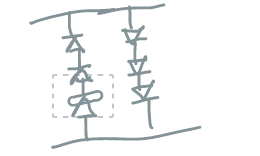
\includegraphics[width=0.8\linewidth]{img/image_2022-09-26-12-36-31.png}
\end{figure}


The hard, squared-off signal response (and multiple of 0.7V) may not be desirable, so we can use a soft limiter instead.


\begin{figure}[H]
	\centering
	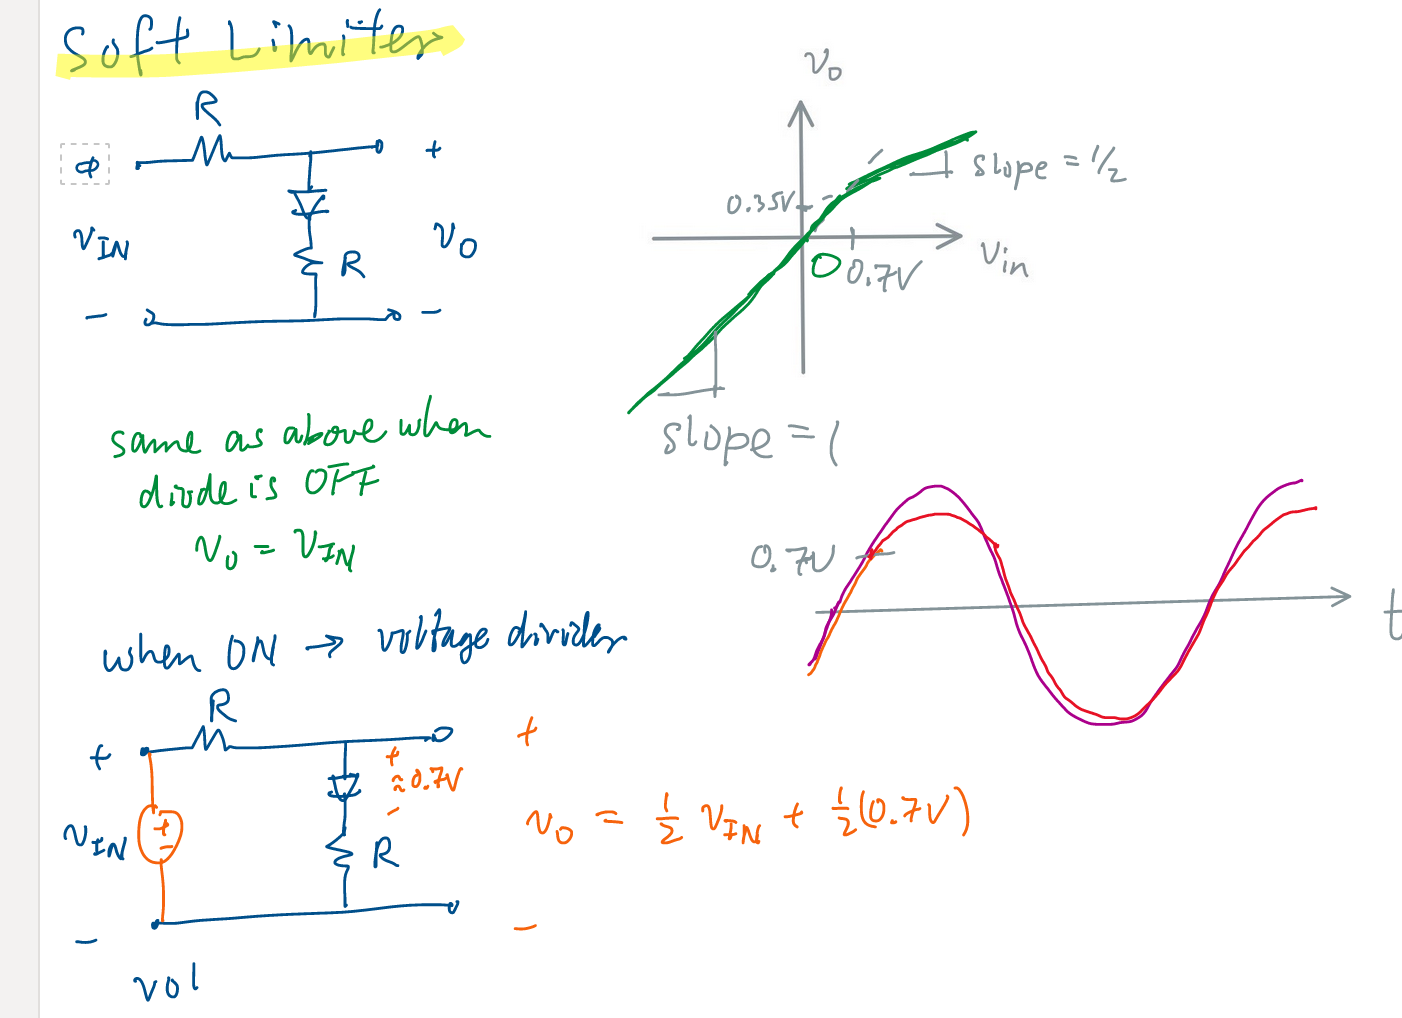
\includegraphics[width=0.8\linewidth]{img/image_2022-09-26-12-37-25.png}
\end{figure}

This will act like nothing is happening when the diode is off, i.e. $ v_o = v_{in}  $. When the diode is on the soft limiting circuit acts like a voltage divider.
For this circuit there are two resistors with the same $ R $ so the output voltage from just the current divider is

\begin{equation}
	v_o = \frac{R}{R+R} v_{in}  = \frac{1}{2} v_{in}
\end{equation}

We will also have to account for the voltage of the diode, so

\begin{equation}
	v_o = \frac{1}{2} v_{in}  + \frac{1}{2} (v_d = 0.7V)
\end{equation}







\begin{equation}
	v_o = \frac{1}{2} v_{in} + \frac{1}{2} 0.7V
\end{equation}



\subsection{Lecture 9}

I missed this lecture, so here are my handwritten catchup notes
\begin{fullpage}
	\begin{figure}[H]
		\centering
		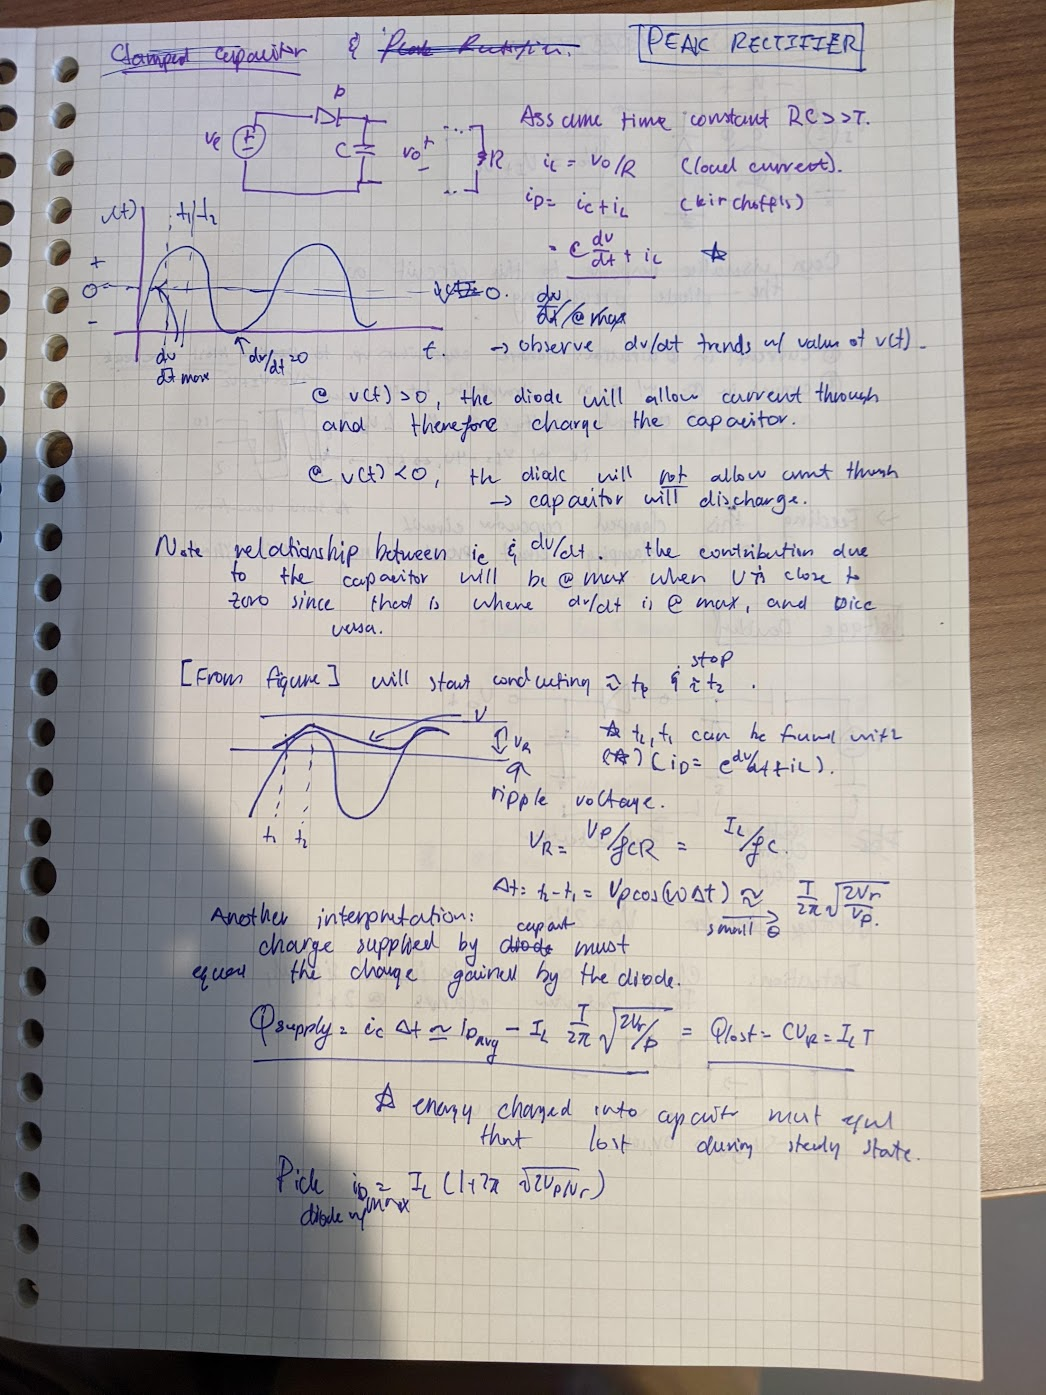
\includegraphics[width=\linewidth]{img/image_2022-09-29-16-36-40.png}
	\end{figure}
\end{fullpage}
\begin{fullpage}
	\begin{figure}[H]
		\centering
		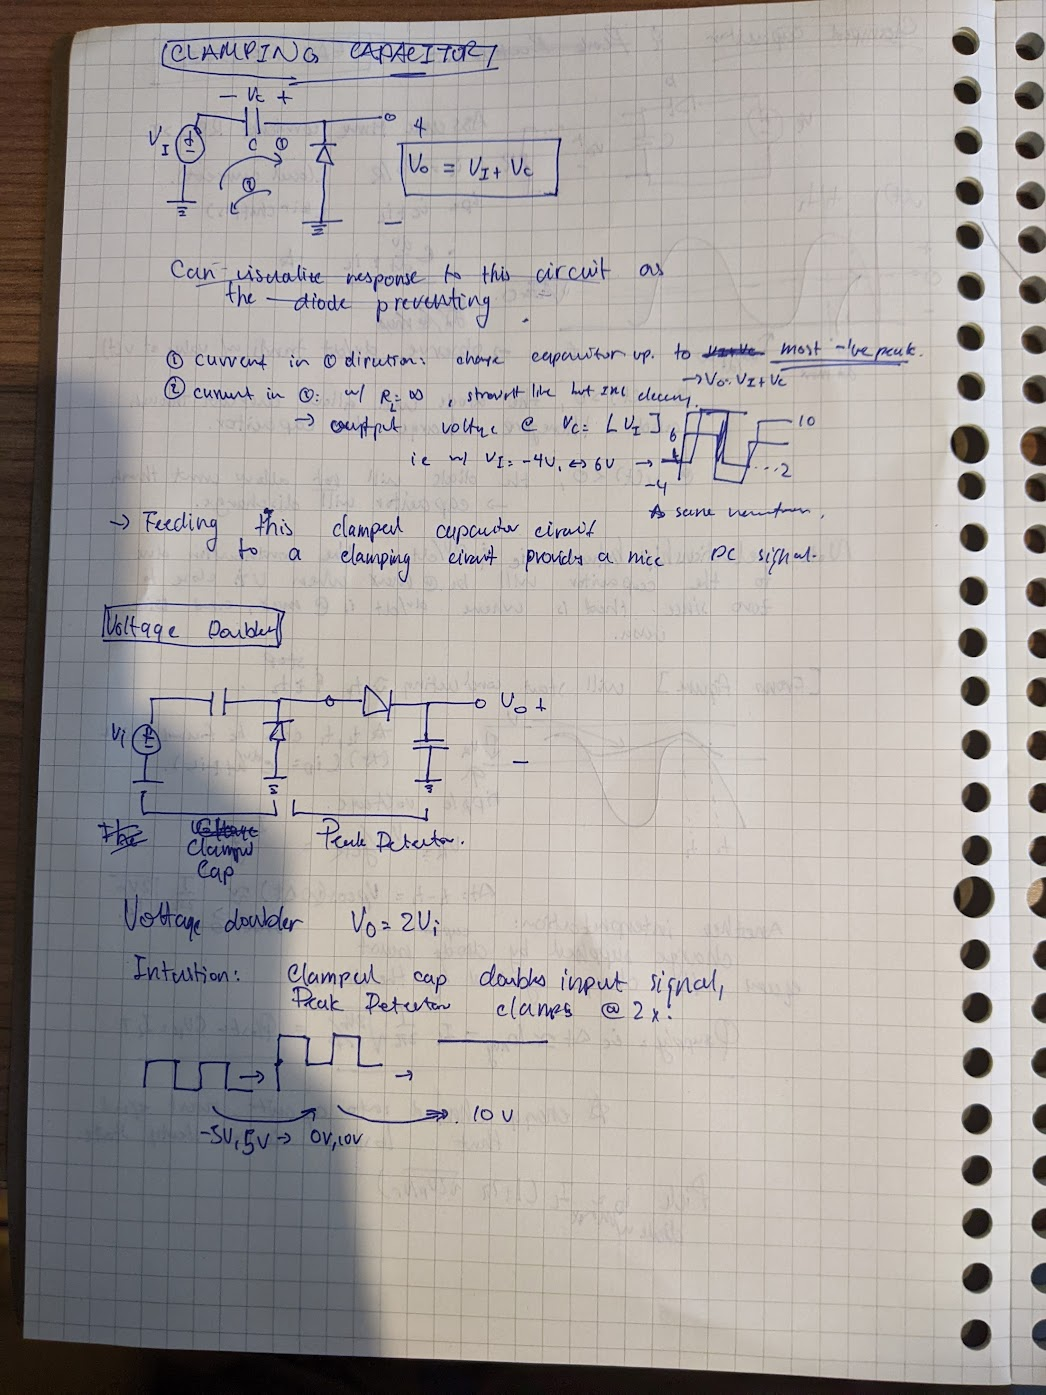
\includegraphics[width=\linewidth]{img/image_2022-09-29-16-36-25.png}
	\end{figure}
\end{fullpage}

\begin{fullpage}
\begin{figure}[H]
	\centering
	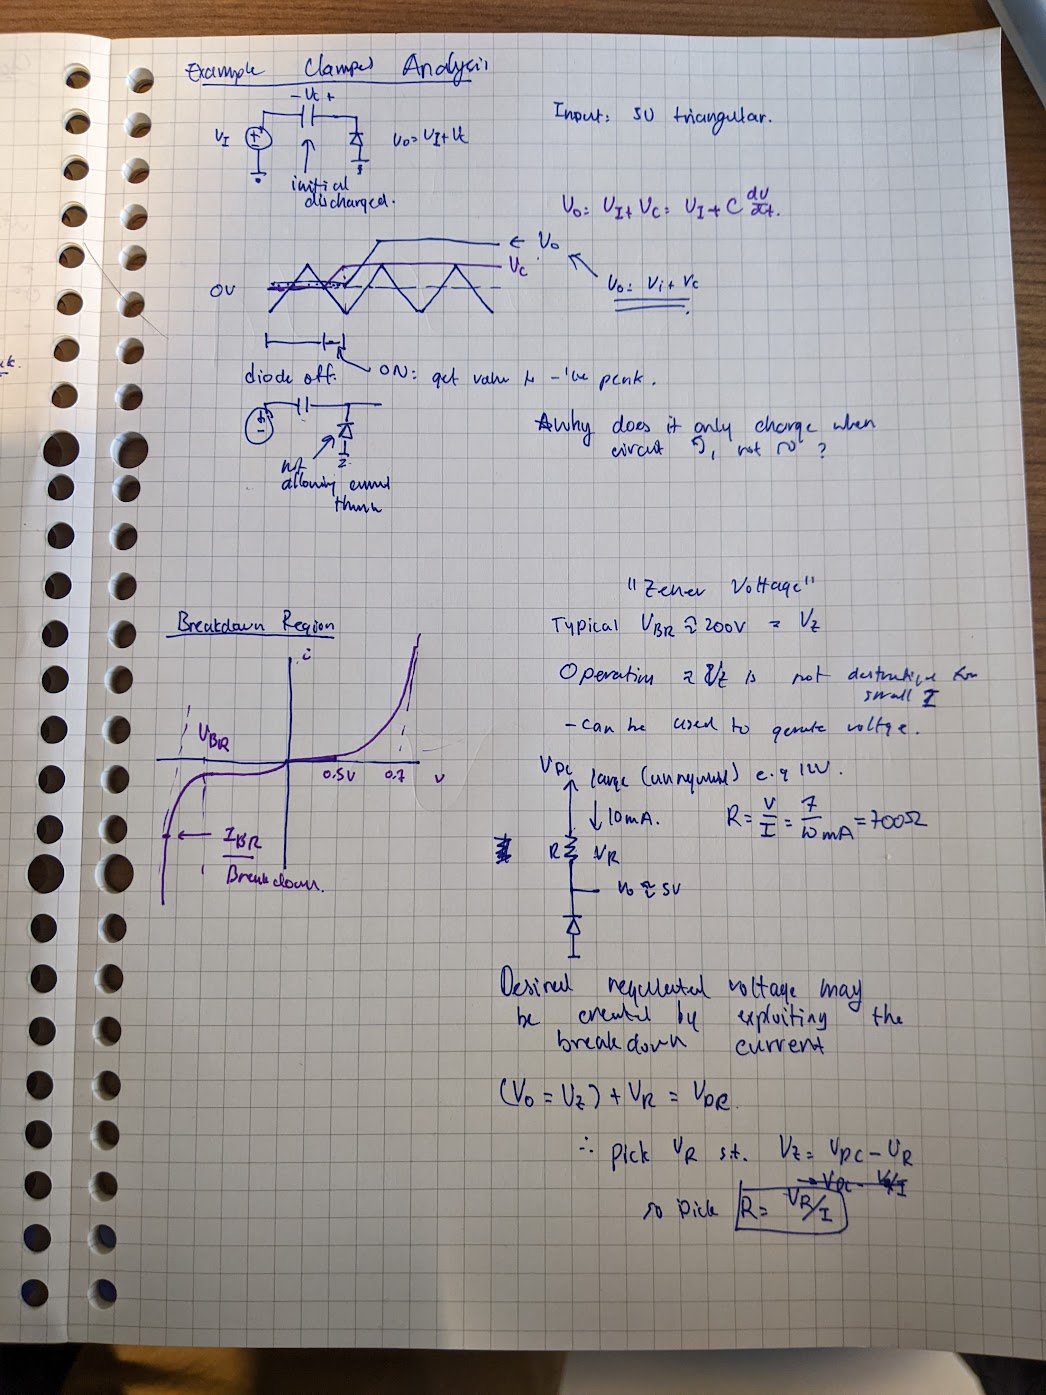
\includegraphics[width=\linewidth]{img/image_2022-09-29-16-34-15.png}
\end{figure}
\end{fullpage}
\end{document}
